%%%%%%%%%%%%%%%%%%%%%%%%%%%%%%%%%%%%
% Lesson Plan (50 minutes)
%%%%%%%%%%%%%%%%%%%%%%%%%%%%%%%%%%%%
\begin{frame}
    \frametitle{Lesson Plan}
    \begin{itemize}
        \item xx min Lecture: Bernoulli distribution, Bernoulli random variables
        \item xx min Edfinity quiz: Bernoulli random variables
        \item xx min Lecture: Geometric distribution, derivation from Bernoulli
        \begin{enumerate}
            \item Probability mass function
            \item Formulas for expectation and variance
            \item Variability
        \end{enumerate}
        \item xx min R Demonstration: sampling from Geometric, different parameters
        \item xx min Edfinity quiz: variability of Geometric random variables
        \item xx min Lecture: review quiz answers
        \item Next time: Binomial (another Bernoulli-linked distribution)
    \end{itemize}
\end{frame}

%%%%%%%%%%%%%%%%%%%%%%%%%%%%%%%%%%%%
% Learning objectives:
%%%%%%%%%%%%%%%%%%%%%%%%%%%%%%%%%%%%
\begin{frame}
    \frametitle{Learning Objectives}
    \begin{itemize}
        \item \textbf{M1 LO3: Use R for Data Management and Exploration:} Utilize R to load, pre-process, and explore data through visualization and summarization techniques.
        \item \textbf{M6 LO1: Validate and Explain Probability Distributions:} Assess the validity of a probability distribution using the concepts of outcome, sample space, and probability properties (e.g., disjoint outcomes, probabilities between 0 and 1, and total probabilities summing to 1).
        \item \textbf{M6 LO4: Understand and Compute Expectations and Variances:} Explain the concepts of expectations and variances of random variables, and compute the expectation and variance of a linear combination of random variables.
        \item \textbf{M6 LO5: Model Data Using Bernoulli, Geometric, and Binomial Distributions:} Recognize when to appropriately model data using the Bernoulli, geometric, and binomial distributions, and compute quantities of interest such as mean, standard deviation, and tail probabilities.
    \end{itemize}
\end{frame}

%%%%%%%%%%%%%%%%%%%%%%%%%%%%%%%%%%%%
% TODO: Copy and adapt these slides base on the lesson plan
%%%%%%%%%%%%%%%%%%%%%%%%%%%%%%%%%%%%

\section{Geometric distribution}

%%%%%%%%%%%%%%%%%%%%%%%%%%%%%%%%%%%%

\subsection{Bernoulli distribution}

%%%%%%%%%%%%%%%%%%%%%%%%%%%%%%%%%%%%

\begin{frame}
\frametitle{Milgram experiment}

\twocol{0.6}{0.4}{

\begin{itemize}

\item Stanley Milgram, a Yale University psychologist, conducted a series of experiments on obedience to authority starting in 1963. 

\item Experimenter (E) orders the teacher (T), the subject of the experiment, to give severe electric shocks to a learner (L) each time the learner answers a question incorrectly. 

\item The learner is actually an actor, and the electric shocks are not real, but a prerecorded sound is played each time the teacher administers an electric shock.

\end{itemize}

}
{
\begin{center}
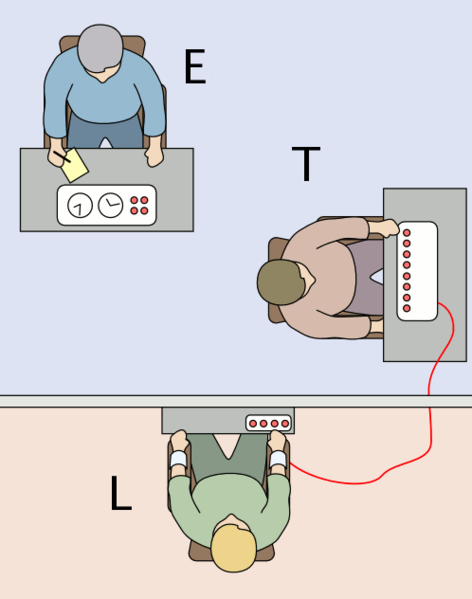
\includegraphics[width=\textwidth]{4-2_geometric_distribution/figures/milgram}
\end{center}
\ct{\webURL{http://en.wikipedia.org/wiki/File:Milgram_Experiment_v2.png}}
}

\end{frame}

%%%%%%%%%%%%%%%%%%%%%%%%%%%%%%%%%%%%

\begin{frame}
\frametitle{Milgram experiment (cont.)}

\begin{itemize}

\item These experiments measured the willingness of study participants to obey an authority figure who instructed them to perform acts that conflicted with their personal conscience.

\item Milgram found that about 65\% of people would obey authority and give such shocks.

\item Over the years, additional research suggested this number is approximately consistent across communities and time.

\end{itemize}

\end{frame}


%%%%%%%%%%%%%%%%%%%%%%%%%%%%%%%%%%%%

\begin{frame}
\frametitle{Bernouilli random variables}

\begin{itemize}

\item Each person in Milgram's experiment can be thought of as a \hl{trial}.

\item A person is labeled a \hl{success} if she refuses to administer a severe shock, and \hl{failure} if she administers such shock.

\item Since only 35\% of people refused to administer a shock, \hl{probability of success} is \mathhl{p = 0.35}.

\item When an individual trial has only two possible outcomes, it is called a \hl{Bernoulli random variable}.

\end{itemize}

\end{frame}

%%%%%%%%%%%%%%%%%%%%%%%%%%%%%%%%%%%%

\subsection{Geometric distribution}

\begin{frame}
\frametitle{Geometric distribution}

{\small

\dq{Dr. Smith wants to repeat Milgram's experiments but she only wants to sample people until she finds someone who will not inflict a severe shock. What is the probability that she stops after the first person?}

\[ P(1^{st}~person~refuses) = 0.35 \]

\pause

\dq{... the third person?}
\[ P(1^{st}~and~2^{nd}~shock,~3^{rd}~refuses) = \slot{S}{0.65} \times \slot{S}{0.65} \times  \slot{R}{0.35} = 0.65^2 \times 0.35 \approx 0.15 \]

\pause

\dq{... the tenth person?}
\soln{
\pause
\[ P(9~shock,~10^{th}~refuses) = \underbrace{\slot{S}{0.65} \times \cdots \times \slot{S}{0.65}}_{9~of~these} \times  \slot{R}{0.35} = 0.65^9 \times 0.35 \approx 0.0072 \]
}
}

\end{frame}

%%%%%%%%%%%%%%%%%%%%%%%%%%%%%%%%%%%%

\begin{frame}
\frametitle{Geometric distribution (cont.)}

\hl{Geometric distribution} describes the waiting time until a success for \hl{independent and identically distributed (iid)} Bernouilli random variables.
\begin{itemize}
\item independence: outcomes of trials don't affect each other
\item identical: the probability of success is the same for each trial
\end{itemize}

$\:$ \\
$\:$ \\

\pause

\formula{Geometric probabilities}{If $p$ represents probability of success, $(1-p)$ represents probability of failure, and $n$ represents number of independent trials \[P(success~on~the~n^{th}~trial) = (1-p)^{n-1} p\]}

\end{frame}

%%%%%%%%%%%%%%%%%%%%%%%%%%%%%%%%%%%%

\begin{frame}

\pq{Can we calculate the probability of rolling a 6 for the first time on the 6$^{th}$ roll of a die using the geometric distribution? Note that what was a success (rolling a 6) and what was a failure (not rolling a 6) are clearly defined and one or the other must happen for each trial.}

\begin{enumerate}[(a)]
\item no, on the roll of a die there are more than 2 possible outcomes
\only<1>{\item yes, why not}
\soln{\only<2>{\item \orange{yes, why not}}}
\end{enumerate}

\soln{
\only<2>{
\[P(6~on~the~6^{th}~roll) = \pr{ \frac{5}{6} }^5 \pr{ \frac{1}{6} } \approx 0.067 \]
}
}

\end{frame}

%%%%%%%%%%%%%%%%%%%%%%%%%%%%%%%%%%%%

\begin{frame}
\frametitle{Expected value}

\dq{How many people is Dr. Smith expected to test before finding the first one that refuses to administer the shock?}

\pause

The expected value, or the mean, of a geometric distribution is defined as $\frac{1}{p}$.
\[ \mu = \frac{1}{p} = \frac{1}{0.35} = 2.86 \]

\pause

She is expected to test 2.86 people before finding the first one that refuses to administer the shock. 

\pause

But how can she test a non-whole number of people?

\end{frame}

%%%%%%%%%%%%%%%%%%%%%%%%%%%%%%%%%%%%

\begin{frame}
\frametitle{Expected value and its variability}

\formula{Mean and standard deviation of geometric distribution}{
\[ \mu = \frac{1}{p} \qquad \qquad \sigma = \sqrt{\frac{1-p}{p^2}} \] 
}

\pause

\begin{itemize}

\item Going back to Dr. Smith's experiment:

\[ \sigma = \sqrt{\frac{1-p}{p^2}} = \sqrt{\frac{1-0.35}{0.35^2}} = 2.3 \]

\pause

\item Dr. Smith is expected to test 2.86 people before finding the first one that refuses to administer the shock, give or take 2.3 people.

\pause

\item These values only make sense in the context of repeating the experiment many many times.

\end{itemize}

\end{frame}

%%%%%%%%%%%%%%%%%%%%%%%%%%%%%%%%%%%%